\documentclass[11pt]{article}

\usepackage[T1]{fontenc}
\usepackage{mathptmx}
\usepackage{graphicx}

\topmargin 0.0in
\setlength{\textwidth} {420pt}
\setlength{\textheight} {620pt} 
\setlength{\oddsidemargin} {20pt}
\setlength{\marginparwidth} {72in}

\usepackage{fancyhdr} 
\usepackage{url}

% set it so that subsubsections have numbers and they
% are displayed in the TOC (maybe hard to read, might want to disable)

\setcounter{secnumdepth}{3}
\setcounter{tocdepth}{3}

% define widow protection

\def\widow#1{\vskip #1\vbadness10000\penalty-200\vskip-#1}

\clubpenalty=10000  % Don't allow orphans
\widowpenalty=10000 % Don't allow widows

% this should give me the ability to use some math symbols that 
% were available by default in standard latex (i.e. \Box)

\usepackage{latexsym}

% define a little section heading that doesn't go with any number

\def\littlesection#1{
\widow{2cm}
\vskip 0.5cm
\noindent{\bf #1}
\vskip 0.0001cm 
}

\pagestyle{fancyplain}

\newcommand{\tstamp}{\today}   
\renewcommand{\sectionmark}[1]{\markright{#1}}
\lhead[\Section \thesection]            {\fancyplain{}{\rightmark}}
\chead[\fancyplain{}{}]                 {\fancyplain{}{}}
\rhead[\fancyplain{}{\rightmark}]       {\fancyplain{}{\thepage}}
\cfoot[\fancyplain{\thepage}{}]         {\fancyplain{\thepage}{}}

\newlength{\myVSpace}% the height of the box
\setlength{\myVSpace}{1ex}% the default, 
\newcommand\xstrut{\raisebox{-.5\myVSpace}% symmetric behaviour, 
  {\rule{0pt}{\myVSpace}}%
}

% leave things with no spacing extra spacing in the final version of the paper
\renewcommand{\baselinestretch}{1.0}    % must go before the begin of doc

% suppress the use of indentation for a paragraph

\setlength{\parindent}{0.0in}
\setlength{\parskip}{0.1in}
\setlength{\headheight}{15pt}

\begin{document}

%% \begin{abstract}

%%   Try

%% \end{abstract}

% handle widows appropriately
\def\widow#1{\vskip #1\vbadness10000\penalty-200\vskip-#1}

% build the title section

\makeatletter

\def\maketitle{%
  %\null
  \thispagestyle{empty}%
  %\vfill
  \begin{center}%\leavevmode
    %\normalfont
    {\Huge \@title\par}%
    %\hrulefill\par
    {\normalsize \@author\par}%
    \vskip .4in
%    {\Large \@date\par}%
  \end{center}%
  %\vfill
  %\null
  %\cleardoublepage

  }

\makeatother

\vspace*{-1.1in}
\title{Pointer Based File Manager to Reduce Data Redundancy and Storage Costs}

% build the author section
\author{Braden D. Licastro\\
Department of Computer Science\\
Allegheny College \\
{\tt licastb@allegheny.edu}  \\
\url{http://www.fullforceapps.com/} \\ 
\vspace*{.1in} \today \\ \vspace*{.1in}
{\bf Abstract} \\ With mass amounts of data being generated every day, the importance of file management technology is becoming ever more prevalent. The average computer user owns approximately 300 gigabytes of data, and in a majority of cases a fair percentage of this is duplicate or irrelevant. To address this problem the research aims to create a pointer based environment that allows files to be accessed easily from numerous locations without creating unnecessary redundancy. Reducing the number of duplicate files benefits the user in numerous ways, from faster response to decreased costs of storage and backups this issue is relevant on numerous fields.}

% use the default title stuff
\maketitle

\vspace*{-.4in}
\section{Introduction}
\label{sec:introduction}
\vspace*{-.1in}

Computers are absolutely everywhere, and society is becoming more digitized every day creating a need for storage of large amount of files. When using a workstation not only are the physical disks in the computer being used but quite possibly hundreds of others around the world. By using this wide array of storage, it becomes easy to build up large amounts of duplicate data. This research will target the problem of data redundancy and provide a solution that will reduce not only storage costs but also inefficiencies. An implementation of a file management system will be introduced that is capable of managing large volumes of files using a database of location pointers and hash keys that identify each individual file. By using pointers, it is possible for the files to be stored on one central location on the disk while avoiding long search times.

By using text based entries in a database, an MD5 hash can be generated for each file in the collection. Because this key is unique for each different file, it is a reliable gauge of uniqueness. When multiple files are found to be identical only one physical copy will be kept but pointers to the database entry will allow easy access. On large network storage servers the benefits become ever more apparent. As users store files on the disks, the system will hash each file and search for a match in a database, thus allowing the user access to the data, but eliminating the overhead of storing numerous copies of identical data. An increase in computation time will exist but should be minimal as text comparisons will be the primary task in finding uniqueness, but this will be outweighed by minimized physical storage requirements and costs of data baskup.

\vspace*{-.1in}
\section{Related Work}
\label{sec:relatedwork}
\vspace*{-.1in}

A significant amount of work exists revolving around data optimization, but the idea of using databases of pointers and hashes to track file location on disk and file uniqueness is mostly undocumented. In addition to a mostly unexplored area of research, many of the data de-duplication methods are very costly when operating on large data sets. The first article to note addresses this issue. The authors set about creating a comparison and detection algorithm that is both fast and efficient. The authors utilized TI-Similarity and RAR methods for quickly scanning the database for potential duplicate records. \cite{Sung:2002:FFS:584792.584808} When a duplicate entry is located it is removed from the collection.

\begin{figure}
\begin{center}
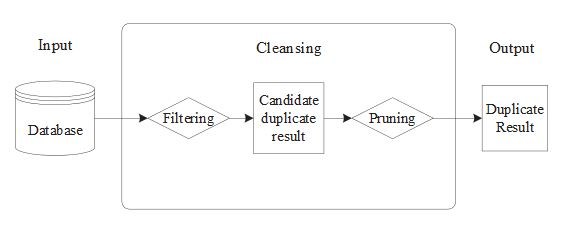
\includegraphics[scale=.8]{duplicate}
\caption{\label{fig:duplicate} The authors' filtering and pruning process.}
\end{center}
\end{figure}

As seen in figure \ref{fig:duplicate}, the database is input into the authors' program and the algorithm searches through the data looking for duplicates. Any duplicate results are evaluated and checked for false positives using the TI-Similarity method. \cite{Sung:2002:FFS:584792.584808} Once a duplicate is validated, the result will be dropped from the database  and the resulting table will be returned and the database state will reflect the changes.

This method of finding duplicate data could be applied to the pointer based file system. By utilixing the authors' RAR and TI-Similarity search methods, it would be more efficient than searching the database one record at a time. The authors used an example table where identical data is inserted into a table by several users. As each entry has its own unique primary key value, the schema was satisfied, but the storage overhead is double what would be needed without redundancy. As seen in figure \ref{fig:duptable} there are three identical entries, their algorithm will remove all but the first occurance leaving the end result of only rows $A$ and $D$.

\begin{figure}
\begin{center}
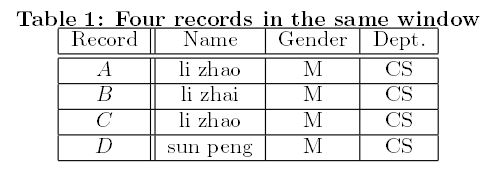
\includegraphics[scale=.8]{duptable}
\caption{\label{fig:duptable} Duplicate entries in the database to be removed.}
\end{center}
\end{figure}

The next authors target the process of removing duplicate files from the physical disk itself. Throughout the paper, they create a framework for finding and removing duplicate file entries located on solid state drives. \cite{Wu:2011:DDA:1982185.1982313} This is extremely valuable for not only the proposed research, but for any real world environment. Solid state drives have a limited number of writes per block of memory, by reducing the number of write requests, not only is the longevity of the disk being improved, but the total consumed space is also reduced therefore allowing more unique data per disk. Solid state drives are inherently fast, so it is possible that the framework, being optimized for said devices, could prove to be highly inefficient on traditional platter based disk drives. The authors track duplicates by the number of references made per file. 

\begin{figure}
\begin{center}
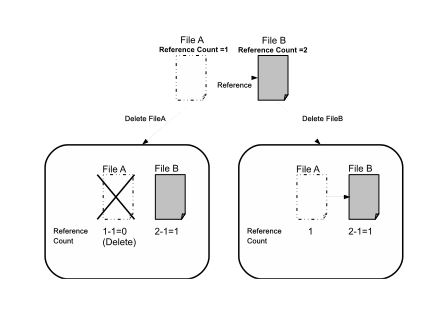
\includegraphics[scale=.8]{delete}
\caption{\label{fig:delete} Authors' file deletion process.}
\end{center}
\end{figure}

As seen in figure \ref{fig:delete}, if a file has a reference count of 0 it will be deleted. If the count is above 0, it cannot be removed as it is still referenced by another file or it is unique. If another file references an older version, the older version will be removed as the latest revision contains the contents of the old file. This method of removal us used in conjunction with perfect matches, as a perfect match is an exact duplicate. The latest modified instance of one of these files is kept, while others are rejected, or if already on disk, will be removed. 

\vspace*{-.2in}
\section{Method of Approach}
\label{sec:method}
\vspace*{-.1in}

In order to implement the proposed research, an open source file manager will need to be acquired and be extended. The file manager must be lightweight and compatible with the linux operating environment. To start, a database will be implemented so that it is able to hold a hashed key and the location of the file on the disk. An example of this schema can be seen in figure \ref{fig:schema}. The software, upon installation will run an initial scan of all user files on the system. The file hash will be generated by running an MD5 hashing function over each file currently on the disk. An INSERT will be run on the database for each file and will record the files current position on the disk, and it will record the result of the hash. Using the searching method outlined by the authors of the first paper in section \ref{sec:relatedwork}, the database will be searched for duplicate hash entries. When a duplicate entry is found, the file manager will remove all but the latest modified entry, and in place of the old modified files, a pointer will be implemented that links to the one remaining file.

In the case of needing duplicate files, so one can be modified while retaining the integrity of the original, it will be possible to open the original using the pointer, but if a saved copy of the file differs from the one that the pointer refers to, the pointer will be overwritten by the new file. This will allow the file system to work as it had before the file manager was implemented, retaining full intuitiveness and flexibility, but data redundancy can be avoided.

\begin{figure}
\begin{center}
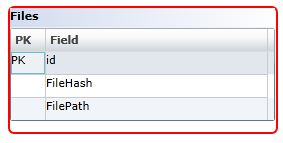
\includegraphics[scale=.8]{schema}
\caption{\label{fig:schema} Example schema to be used.}
\end{center}
\end{figure}

\vspace*{-.2in}
\section{Evaluation Strategy}
\label{sec:evaluate}
\vspace*{-.1in}

Evaluating the effectiveness of the program will entail several benchmark readings. The total number of files, the number of unique files, and the overall percentage of the disk will be evaluated to determine the effectiveness of the file manager. The total number of files will be fixed for every test run and the files used will be exactly the same for each run. The number of files will be the total number of files on the system located inside of the test file structure. This will not include program or system files. The number of duplicates will be randomly generated initially and the same file structure will be used each time the experiment is run. Duplicates are defined as files with identical metadata and contents. The total disk space utilized will be determined by measuring the total size of the file structure containing the test structure.

Again, the same tests will be performed, but will be run with the proposed file management system. After the initial running of the program, statistics will be gathered that include the total run time of the program to completion, the final number of files, the number of remaining duplicate files, and the total storage space used. Because the system implements a text based database, the total storage space will be reduced, but the efficiency of the system will need to be determined.

\vspace*{-.1in}
\section{Research Schedule}
\label{sec:schedule}
\vspace*{-.1in}

The research schedule for the project is to be tentatively based off of the following deadlines. Due to the nature of the project and the wide array of pre-existing software required needing to be modified and implemented, unseen hurdles may arise. 

Phase 1 - 1 month: Find acceptable open source operating system and file manager. Begin the process of learning libraries and code so implementation can begin.

Phase 2 - 2-3 months: Develop a working program which is capable of satisfying the requirements outlined in section \ref{sec:method}. Set up a basic file structure to be used as a baseline for the research project. Record the number of files, number of duplicates, and the total storage space used compared to the file system with no user generated files.

Phase 3 - 1 week: During this time I will run various tests on the program using the proposed methods in section \ref{sec:method} and record the results of the experiment. Results to be recorded are the final number of files, the number of remaining duplicates, and the total storage space used.

Phase 4 - remaining time: The results gathered throughout the test process will be evaluated and the software tweaked and finalized. After modifications are complete tests will be rerun and the final results will be evaluated.

\vspace*{-.1in}
\section{Conclusion}
\label{sec:conclusion}
\vspace*{-.1in}

With computers becoming ever more prevalent and data being generated at an exponential rate, it is becoming more and more necessary every day to reduce the redundancy and create a more efficient file system. By removing duplicate files from a system while retaining structure and organization this problem can be addressed and will not only reduce the amount of storage space required, but can also improve search efficiency by using stored information in a database and also reduce time spent sorting through structures manually removing duplicate data before backups.

\bibliographystyle{plain}
\bibliography{senior_thesis_proposal}

\end{document}

